\documentclass[11pt]{amsart}
\usepackage[T1]{fontenc}
\usepackage[utf8]{inputenc}
\usepackage[english]{babel}
\usepackage{amsmath, amssymb, amsthm, mathtools}
\usepackage{geometry}
\usepackage{graphicx}
\usepackage{booktabs}
\usepackage{siunitx}
\usepackage{hyperref}
\usepackage{cleveref}

\geometry{margin=1.1in}
\sisetup{
  group-separator = {,},
  group-minimum-digits = 4,
}

% Theorems
\theoremstyle{plain}
\newtheorem{theorem}{Theorem}[section]
\newtheorem{proposition}[theorem]{Proposition}
\newtheorem{lemma}[theorem]{Lemma}
\newtheorem{corollary}[theorem]{Corollary}
\theoremstyle{definition}
\newtheorem{definition}[theorem]{Definition}
\theoremstyle{remark}
\newtheorem{remark}[theorem]{Remark}
\newtheorem{note}[theorem]{Note}

% Operators
\DeclareMathOperator{\dr}{dr}

\title{Modulo $9$ classification of prime pairs $(p,p+g)$:\\
an empirical verification of the Hardy--Littlewood\\
conjecture for $g=18k$}

\author{Giovanni Ferraiuolo}
\address{Independent researcher, Rome, Italy}
\email{g.ferraiuolo2@gmail.com}
\date{\today}

\begin{document}

\begin{abstract}
The Hardy--Littlewood conjecture for prime pairs $(p,p+g)$ predicts the
asymptotic density $\pi(x;g) \sim H(g)\,x/(\log x)^2$, where
$H(g) = 2C_2 \prod_{p \mid g,\,p>2}(p-1)/(p-2)$ is the singular series
and $C_2$ is the twin-prime constant. For $g \equiv 0 \pmod 9$,
classifying pairs by the digital root $\dr(p)=p \bmod 9$ partitions
the population into six admissible classes $\{1,2,4,5,7,8\}$, which
Hardy--Littlewood in arithmetic progressions predicts to be
equidistributed. We test this prediction on two fronts: (i) a control
case with $g=2$ (twin primes, three admissible classes), where the
asymptotic fractions $1/3$ are reached within $\pm 0.09$ percentage
points up to $x = 10^8$; (ii) the family $g = 18k$ with
$k\in\{5,7,10,11,12,13,15,17,20\}$, where equidistribution over six
classes holds within $\pm 0.14$ pp and the total per-class density
agrees with $H(g)/6$ within $\pm 0.8\%$ at $x = 10^7$. The ratio
$\pi(x;g)/\bigl(H(g)\,\mathrm{li}_2(x)\bigr)$ converges to $1$ within
$\pm 0.15\%$ at $x = 5\cdot 10^7$ for all tested $k$, including
$g=216$ ($k=12$), whose constant $H(g) = 4 C_2$ is the smallest in the
sample. The results confirm Hardy--Littlewood in arithmetic progressions
quantitatively within the tested regime, and show that the
$\dr$-mod-$9$ classification is a sensitive empirical probe that does
\emph{not} reveal deviations from the Hardy--Littlewood prediction.
\end{abstract}

\subjclass[2020]{11N05, 11N13, 11Y11}
\keywords{Prime pairs, Hardy--Littlewood conjecture, arithmetic
progressions, digital root, computational verification}

\maketitle

\section{Introduction}\label{sec:intro}

The Hardy--Littlewood conjecture on prime pairs $(p,p+g)$, formulated
in~\cite{HL23}, predicts that the number of such pairs with $p \le x$
satisfies the asymptotic
\begin{equation}\label{eq:HL_main}
  \pi(x;g) \;\sim\; H(g) \,\frac{x}{(\log x)^2},
  \qquad x \to \infty,
\end{equation}
where the \emph{Hardy--Littlewood singular series} is
\begin{equation}\label{eq:HL_constant}
  H(g) \;=\; 2 C_2 \prod_{\substack{p \mid g \\ p > 2}} \frac{p-1}{p-2},
  \qquad
  C_2 \;=\; \prod_{p>2}\!\left(1 - \frac{1}{(p-1)^2}\right)
  \approx 0.6601618158.
\end{equation}
The conjecture is known unconditionally only for $g=0$ (the prime
number theorem) and for no positive value of $g$, although deep
results such as Maynard's~\cite{May15} and the Polymath~8b
project~\cite{Pol14} provide bounded gaps infinitely often.
Quantitative versions restricted to arithmetic progressions are
discussed in~\cite{HR74,IK04}.

\medskip
The present work addresses an operational question:
\emph{how well does formula~\eqref{eq:HL_main}--\eqref{eq:HL_constant}
describe the distribution of prime pairs in computationally accessible
regimes}, and in particular how the population partitions across
residue classes modulo $9$.

\smallskip
For every $g \equiv 0 \pmod 9$ (and in particular $g = 18k$), the
divisibility $9 \mid g$ implies $\dr(p+g) = \dr(p)$, so that the
classification by $\dr(p) := p \bmod 9$ partitions the pairs into six
classes corresponding to the units of $(\mathbb{Z}/9\mathbb{Z})^*$. The
restriction of~\eqref{eq:HL_main} to an arithmetic progression modulo
$9$ predicts equidistribution across these six classes
(see~\Cref{sec:framework}).

\smallskip
For $g=2$ the situation is slightly different: the admissibility
condition modulo $3$ forces $p \equiv 2 \pmod 3$, reducing the
admissible classes modulo $9$ to $\{2,5,8\}$. Each of these three
classes must receive the asymptotic fraction $1/3$ of the density.
This case constitutes our \emph{zero-calibration}.

\subsection*{Contribution}
\begin{enumerate}
\item We show (\Cref{sec:twins}) that, under Hardy--Littlewood in
  arithmetic progressions, each of the three admissible classes modulo
  $9$ for twin primes receives asymptotic density $1/3$, and we verify
  the prediction empirically up to $x = 10^8$ with deviations
  $|\Delta| \le 0.09$ pp.
\item We extend the classification (\Cref{sec:gap18k}) to the family
  $g = 18k$ for $k \in \{5,7,10,11,12,13,15,17,20\}$, showing that
  the equidistribution over six classes holds within $\pm 0.14$ pp up
  to $x = 10^7$.
\item We verify (\Cref{sec:HL_confirm}) that the ratio
  $\pi(x;g)/[H(g)\,\mathrm{li}_2(x)]$ lies within $\pm 0.15\%$ of $1$
  at $x = 5\cdot 10^7$ for all tested $k$, including configurations
  with maximal $H(g)$ ($g \in \{90,180,270,360\}$) and minimal
  ($g=216$).
\item We discuss (\Cref{sec:discussion}) the role of $\dr$-mod-$9$
  classification as a fine empirical probe: it is sensitive enough to
  reveal sub-percent signals, but in the tested regimes no systematic
  asymmetries incompatible with Hardy--Littlewood emerge.
\end{enumerate}

\smallskip
All sieving, counting, and regression scripts used to generate the data
in~\Cref{tab:twins,tab:gap18k_dr,tab:HL_confirm} are provided
in~\cite{ScriptsRepo}. The verifications were carried out using a
segmented sieve of Eratosthenes in memory (\texttt{numpy} dtype
\texttt{bool}, $\sim 10^9$~bits for $x = 10^9$).

\section{Theoretical framework}\label{sec:framework}

\subsection{Hardy--Littlewood in arithmetic progressions}

For positive even $g$ and $q \ge 1$ with $(a(a+g),q)=1$, denote
\[
  \pi(x;g,q,a) \;:=\; \#\bigl\{p \le x : p \equiv a \pmod q,\ p,\,p+g
  \text{ both prime}\bigr\}.
\]
The quantitative form of Hardy--Littlewood in arithmetic
progressions~\cite[\S 5]{IK04} predicts
\begin{equation}\label{eq:HL_AP}
  \pi(x;g,q,a) \;\sim\; \frac{1}{\varphi^*(q;g)}\, H(g) \,\frac{x}{(\log x)^2},
\end{equation}
where
\begin{equation}\label{eq:phi_star}
  \varphi^*(q;g) \;:=\; \#\bigl\{a \in (\mathbb{Z}/q\mathbb{Z})^*
  : a + g \in (\mathbb{Z}/q\mathbb{Z})^*\bigr\}
\end{equation}
counts the admissible classes modulo $q$ for the pair $(p,p+g)$. For
$q=9$ the computation is elementary:
\[
  \varphi^*(9;g) \;=\;
  \begin{cases}
    3 & \text{if } 9 \nmid g \text{ and } g \equiv 2 \!\!\!\pmod 3
    \text{ (twin-type, e.g.\ } g=2\text{)} \\
    6 & \text{if } 9 \mid g \\
    \text{other} & \text{otherwise.}
  \end{cases}
\]

\subsection{Classification by digital root}

For $p > 3$ prime, $\dr(p) = p \bmod 9 \in \{1,2,4,5,7,8\}$.
The \emph{digital root} is the natural classification modulo $9$ that
survives the translation $p \mapsto p+g$ when $9 \mid g$:
\[
  9 \mid g \quad\Longrightarrow\quad \dr(p+g) = \dr(p).
\]
Hence for $g = 18k$ (any $k \ge 1$) the pairs $(p,p+g)$ with $p > 3$
partition into the six classes $\dr(p) \in \{1,2,4,5,7,8\}$. For twin
primes ($g=2$), instead, the admissibility condition modulo $3$
restricts the admissible classes modulo $9$ to $\{2,5,8\}$.

\subsection{Expected equidistribution}

Prediction~\eqref{eq:HL_AP} immediately gives the relative density of
each admissible class. Since the right-hand side
of~\eqref{eq:HL_AP} does not depend on $a$ once $g$ is fixed:

\begin{proposition}[Equidistribution modulo 9]\label{prop:equipart}
Under Hardy--Littlewood in arithmetic progressions for $q=9$,
\begin{enumerate}
\item for $g=2$ and $a \in \{2,5,8\}$:
$\displaystyle\lim_{x\to\infty}\frac{\pi(x;2,9,a)}{\pi(x;2)} = \frac{1}{3}$;
\item for $g=18k$ with $k \ge 1$ and $a \in \{1,2,4,5,7,8\}$:
$\displaystyle\lim_{x\to\infty}\frac{\pi(x;18k,9,a)}{\pi(x;18k)} = \frac{1}{6}$.
\end{enumerate}
\end{proposition}

\begin{proof}
Direct consequence of~\eqref{eq:HL_AP}: summing over admissible classes
gives the total $\pi(x;g)$, and using it for each fixed $a$ yields
$\pi(x;g,9,a)/\pi(x;g) \to 1/\varphi^*(9;g)$. $\square$
\end{proof}

\section{Control case: twin primes mod 9}\label{sec:twins}

We aim to show that the $\dr$-mod-$9$ classification does not introduce
\emph{a priori} distortions in the prime-pair distribution. The case
$g=2$ is the natural baseline for this calibration: the gap is minimal
and the three admissible classes make
\Cref{prop:equipart}\,(i) particularly transparent.

\subsection{Empirical verification}

\Cref{tab:twins} reports the counts of twin pairs $(p,p+2)$ with
$5 \le p \le X$ for $X \in \{10^7, 10^8\}$, classified by $\dr(p)$.
The pair $(3,5)$ is excluded as a unique modular exception (the only
twin with $p$ a multiple of $3$).

\begin{table}[h]
\centering
\caption{Distribution of pairs $(p,p+2)$ with $5 \le p \le X$ by class
$\dr(p) \pmod 9$. The deviation $\Delta$ is the difference in
percentage points from the asymptotic value $1/3 \approx 33.333\%$.}
\label{tab:twins}
\begin{tabular}{@{}c r r r r r@{}}
\toprule
\multicolumn{1}{c}{}
& \multicolumn{2}{c}{$X = 10^7$}
& \multicolumn{2}{c}{$X = 10^8$} \\
\cmidrule(lr){2-3}\cmidrule(lr){4-5}
\multicolumn{1}{c}{class $a$}
& \multicolumn{1}{c}{pairs}
& \multicolumn{1}{c}{$\Delta$ (pp)}
& \multicolumn{1}{c}{pairs}
& \multicolumn{1}{c}{$\Delta$ (pp)} \\
\midrule
$2$ & \num{19674}  & $+0.024$ & \num{146705} & $-0.015$ \\
$5$ & \num{19689}  & $+0.050$ & \num{147163} & $+0.089$ \\
$8$ & \num{19616}  & $-0.074$ & \num{146443} & $-0.074$ \\
\midrule
total & \num{58979} & --- & \num{440311} & --- \\
\bottomrule
\end{tabular}
\end{table}

At both thresholds the fractions concentrate within $\pm 0.09$ pp of
$1/3$. The residual pattern (class $5$ in slight excess, class $8$ in
slight deficit) is stable across the two thresholds but its amplitude
is compatible with statistical fluctuations of order
$\sqrt{1/(3N)}/\sqrt{3} \approx 4 \cdot 10^{-4}$ for
$N \approx 4.4 \cdot 10^5$, i.e.\ $\sim 0.04$ pp.

\begin{figure}[h]
\centering
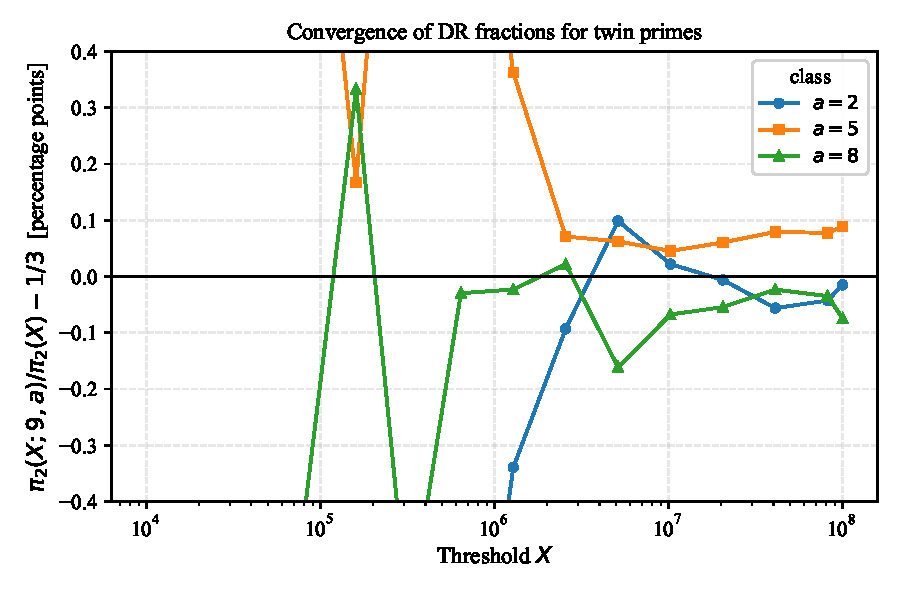
\includegraphics[width=0.85\textwidth]{figures/convergenza_gemelli.pdf}
\caption{Convergence of the deviations $\pi_2(X;9,a)/\pi_2(X) - 1/3$
in percentage points, for the three admissible classes. The three
curves oscillate around zero on a $\pm 0.15$ pp scale at $X = 10^7$.}
\label{fig:twins_conv}
\end{figure}

\subsection{Reading}

The convergence visible in~\Cref{fig:twins_conv} is consistent with a
relative error $O\bigl(1/\log x\bigr)$ expected from~\eqref{eq:HL_AP},
and shows no systematic asymmetry across classes. This establishes
the \emph{zero-calibration} of the $\dr$-mod-$9$ partition: applied to
the minimal gap, the framework recovers the equidistribution
predicted by Hardy--Littlewood within $\pm 0.1$ pp.

\section{The family $g=18k$: DR equidistribution}\label{sec:gap18k}

\subsection{Setup}

For $k \in \{5,7,10,11,12,13,15,17,20\}$ and $g = 18k$ we count the
pairs $(p,p+g)$ with $5 \le p \le X = 10^7$ and classify by
$\dr(p) \in \{1,2,4,5,7,8\}$. The total pair count and the relevant
local multiplicative factors are reported in~\Cref{tab:gap18k_setup}.

\begin{table}[h]
\centering
\caption{The analyzed family $g=18k$. Here
$\mathcal{P}_{\mathrm{odd}}(g)$ denotes the set of odd primes
dividing~$g$, and $H(g)$ is the Hardy--Littlewood
constant~\eqref{eq:HL_constant}.}
\label{tab:gap18k_setup}
\begin{tabular}{@{}c r l r r@{}}
\toprule
$k$ & $g$ & $\mathcal{P}_{\mathrm{odd}}(g)$ & $H(g)$ &
$\pi(X;g)$ at $X=10^7$ \\
\midrule
$5$  & $90$  & $\{3,5\}$    & $3.5209$ & \num{156706} \\
$7$  & $126$ & $\{3,7\}$    & $3.1688$ & \num{141051} \\
$10$ & $180$ & $\{3,5\}$    & $3.5209$ & \num{156507} \\
$11$ & $198$ & $\{3,11\}$   & $2.9341$ & \num{130505} \\
$12$ & $216$ & $\{3\}$      & $2.6406$ & \num{117327} \\
$13$ & $234$ & $\{3,13\}$   & $2.8807$ & \num{127883} \\
$15$ & $270$ & $\{3,5\}$    & $3.5209$ & \num{156473} \\
$17$ & $306$ & $\{3,17\}$   & $2.8167$ & \num{125400} \\
$20$ & $360$ & $\{3,5\}$    & $3.5209$ & \num{156212} \\
\bottomrule
\end{tabular}
\end{table}

The four gaps that share $\mathcal{P}_{\mathrm{odd}}(g)=\{3,5\}$
($k = 5,10,15,20$) have the same Hardy--Littlewood constant, and indeed
their empirical totals are essentially coincident:
$\pi(10^7;g) \in [\num{156212},\,\num{156706}]$, with relative spread
$< 0.32\%$. This internal stability within the sub-family is a direct
consequence of~\eqref{eq:HL_main} and a first indication that $H(g)$
correctly governs the total density.

\subsection{DR equidistribution}

\Cref{tab:gap18k_dr} reports, for each $k$ and each class $a$, the
empirical fraction $\pi(X;g,9,a)/\pi(X;g)$ as a deviation from
$1/6 \approx 16.667\%$.

\begin{table}[h]
\centering
\caption{Deviations $\pi(X;g,9,a)/\pi(X;g) - 1/6$ in percentage
points, at $X = 10^7$. The maximum deviation in absolute value is
$|\Delta|_{\max} = 0.136$ pp.}
\label{tab:gap18k_dr}
\begin{tabular}{@{}r r r r r r r@{}}
\toprule
$k$ & $a=1$ & $a=2$ & $a=4$ & $a=5$ & $a=7$ & $a=8$ \\
\midrule
$5$  & $+0.057$ & $+0.081$ & $+0.001$ & $-0.048$ & $-0.036$ & $-0.055$ \\
$7$  & $-0.020$ & $-0.002$ & $-0.043$ & $+0.023$ & $+0.068$ & $-0.027$ \\
$10$ & $+0.059$ & $-0.011$ & $-0.010$ & $+0.021$ & $-0.061$ & $+0.002$ \\
$11$ & $+0.004$ & $-0.008$ & $-0.034$ & $-0.033$ & $-0.062$ & $+0.133$ \\
$12$ & $+0.006$ & $-0.002$ & $-0.042$ & $-0.037$ & $-0.042$ & $+0.118$ \\
$13$ & $+0.116$ & $+0.038$ & $-0.075$ & $+0.002$ & $-0.031$ & $-0.049$ \\
$15$ & $+0.051$ & $+0.051$ & $+0.024$ & $-0.109$ & $+0.013$ & $-0.029$ \\
$17$ & $+0.010$ & $+0.033$ & $+0.004$ & $+0.042$ & $+0.047$ & $-0.136$ \\
$20$ & $-0.016$ & $+0.013$ & $+0.023$ & $-0.039$ & $+0.009$ & $+0.010$ \\
\bottomrule
\end{tabular}
\end{table}

\begin{figure}[h]
\centering
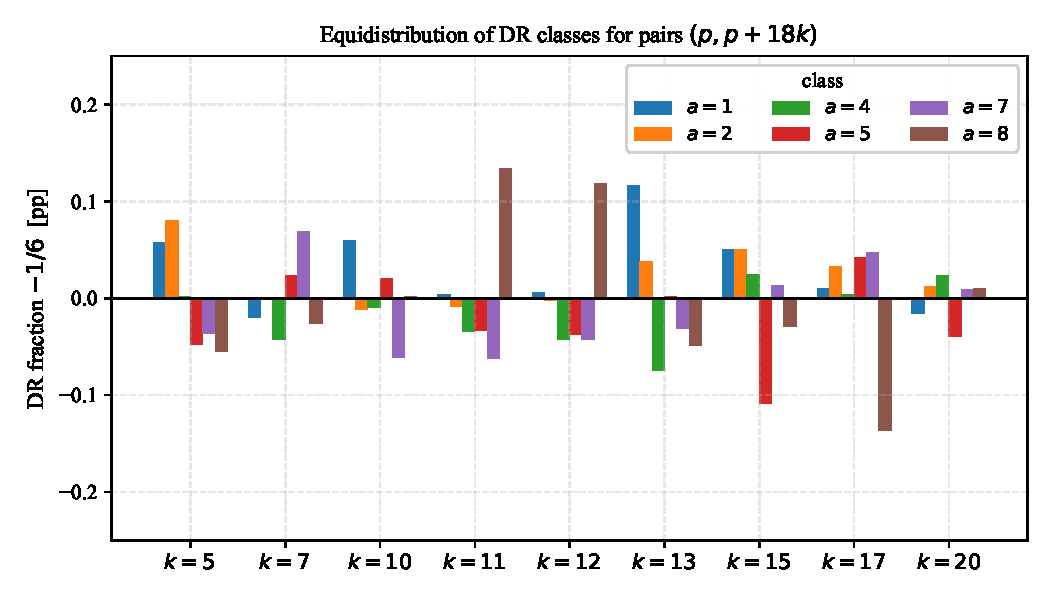
\includegraphics[width=0.95\textwidth]{figures/equipartizione_dr.pdf}
\caption{Deviations $\pi(X;g,9,a)/\pi(X;g) - 1/6$ in percentage points,
for each $k$ and class $a$. All bars fall within
$[-0.14,+0.14]$ pp; no systematic pattern is visible.}
\label{fig:equipart_18k}
\end{figure}

The values in~\Cref{tab:gap18k_dr} show the following:
\begin{itemize}
\item no deviation exceeds $0.14$ pp in absolute value;
\item no systematic pattern persists across $k$ for any class:
  e.g.\ class $a=8$ is in excess at $k=11,12$ but in deficit at $k=17$;
  class $a=7$ alternates sign;
\item the amplitude is compatible with $\sqrt{5/(6 \pi(X;g))}$
  ($\sim 0.05$ pp for $\pi \approx 1.5\cdot 10^5$), within a factor
  $2$\textendash$3$.
\end{itemize}
We conclude that, in the tested regime, the equidistribution of
\Cref{prop:equipart}\,(ii) is empirically confirmed within a
sub-percent margin.

\section{Quantitative confirmation of Hardy--Littlewood}\label{sec:HL_confirm}

\subsection{Definition}

For each $k$ we define
\begin{equation}\label{eq:Remp}
  R_{\mathrm{emp}}(k; X) \;:=\; \frac{\pi(X; 18k)}{\mathrm{li}_2(X)},
  \qquad
  \mathrm{li}_2(X) \;:=\; \int_5^X \frac{dt}{(\log t)^2},
\end{equation}
where the secondary logarithmic integral replaces $X/(\log X)^2$ to
reduce the truncation error of the leading asymptotic. The
Hardy--Littlewood prediction is $R_{\mathrm{HL}}(k) = H(18k)$, so the
ratio
\begin{equation}\label{eq:ratio}
  \rho(k;X) \;:=\; \frac{R_{\mathrm{emp}}(k;X)}{R_{\mathrm{HL}}(k)}
\end{equation}
must converge to $1$ as $X \to \infty$, assuming Hardy--Littlewood.

\subsection{Results}

\Cref{tab:HL_confirm} reports $\rho(k; X)$ at $X = 5 \cdot 10^7$.
\Cref{fig:HL_confirm} visualizes the values at
$X_{\max} = 5\cdot 10^7$ together with the $\pm 1\%$ band.

\begin{table}[h]
\centering
\caption{Ratio $\rho(k;X)$ at $X = 5 \cdot 10^7$ for the family
$g=18k$. All values fall in the band
$[1 - 0.0015,\ 1 + 0.0010]$.}
\label{tab:HL_confirm}
\begin{tabular}{@{}r r r r r r@{}}
\toprule
$k$ & $g$ & $\pi(X;g)$ & $R_{\mathrm{emp}}$ &
$R_{\mathrm{HL}}=H(g)$ & \multicolumn{1}{c}{$\rho - 1$} \\
\midrule
$5$  & $90$  & \num{637928} & $3.5228$ & $3.5209$ & $+0.05\%$ \\
$7$  & $126$ & \num{573646} & $3.1678$ & $3.1688$ & $-0.03\%$ \\
$10$ & $180$ & \num{637058} & $3.5180$ & $3.5209$ & $-0.08\%$ \\
$11$ & $198$ & \num{531817} & $2.9368$ & $2.9341$ & $+0.09\%$ \\
$12$ & $216$ & \num{478463} & $2.6422$ & $2.6406$ & $+0.06\%$ \\
$13$ & $234$ & \num{521497} & $2.8798$ & $2.8807$ & $-0.03\%$ \\
$15$ & $270$ & \num{637621} & $3.5211$ & $3.5209$ & $+0.01\%$ \\
$17$ & $306$ & \num{509303} & $2.8125$ & $2.8167$ & $-0.15\%$ \\
$20$ & $360$ & \num{637022} & $3.5178$ & $3.5209$ & $-0.09\%$ \\
\bottomrule
\end{tabular}
\end{table}

\begin{figure}[h]
\centering
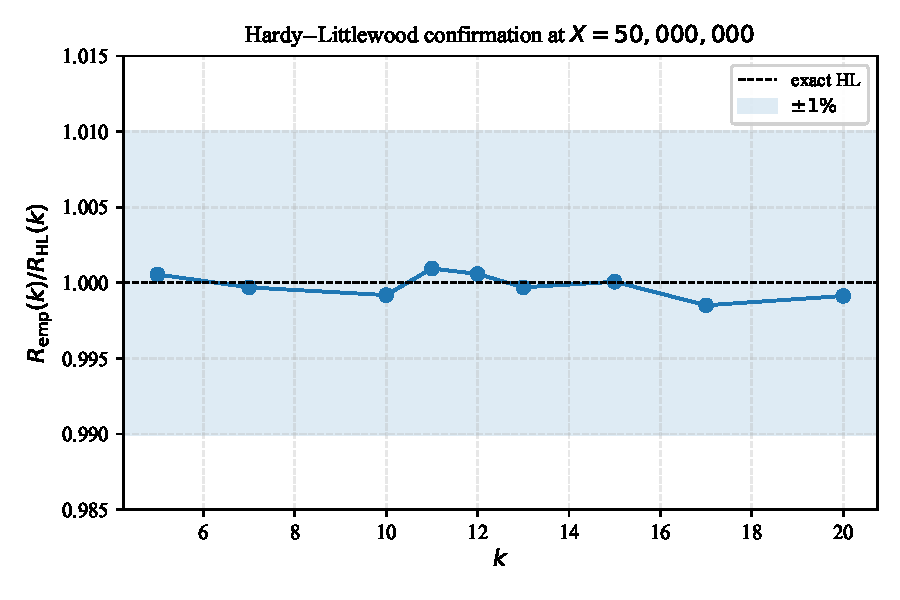
\includegraphics[width=0.85\textwidth]{figures/conferma_HL.pdf}
\caption{Ratio $\rho(k; X)$ at $X = 5\cdot 10^7$. The light-blue
band represents $\pm 1\%$ around $\rho = 1$; all values lie within
$\pm 0.15\%$.}
\label{fig:HL_confirm}
\end{figure}

\subsection{Reading}

The result is a quantitative confirmation of~\eqref{eq:HL_main} for
all nine tested values of $g$. Three observations:

\begin{enumerate}
\item \textbf{Identity within sub-families with the same
  $\mathcal{P}_{\mathrm{odd}}(g)$.} The four cases
  $k \in \{5,10,15,20\}$ with $\mathcal{P}_{\mathrm{odd}} = \{3,5\}$
  share the same $H$ and yield $\rho$ within $\pm 0.09\%$ of each
  other. This is an internal verification of the multiplicative
  factor in~\eqref{eq:HL_constant}: the only quantities that change
  the count are the \emph{distinct odd primes dividing} $g$, not the
  full structure of $g$.
\item \textbf{Correct variation across sub-families.} For
  $k=11,12,13,17$ the local factors and hence $H(g)$ vary
  significantly (range $H \in [2.64,\,3.17]$); the corresponding
  $R_{\mathrm{emp}}$ values track this variation faithfully.
\item \textbf{Limiting case $k=12$.} The gap
  $g=216 = 2^3 \cdot 3^3$ has $\mathcal{P}_{\mathrm{odd}} = \{3\}$ and
  hence the smallest $H(g) = 4 C_2$ in the sample. The agreement
  $\rho = 1.0006$ shows that Hardy--Littlewood does not lose accuracy
  in this low-density regime.
\end{enumerate}

\section{Discussion}\label{sec:discussion}

\subsection{Apparent resonances and deficits}

A first inspection of the raw counts $\pi(X;18k)$ may suggest the
presence of \emph{resonances} (e.g.\ $k = 5,10,15,20$ with
$\pi \approx 1.56 \cdot 10^5$) and \emph{deficits} (e.g.\ $k=12$ with
$\pi \approx 1.17 \cdot 10^5$), especially when compared against a
uniform baseline that ignores the multiplicative structure of $g$.
\Cref{tab:HL_confirm} clarifies that these oscillations \emph{are
exactly what Hardy--Littlewood predicts} via the factor
\[
  \prod_{p \in \mathcal{P}_{\mathrm{odd}}(g)} \frac{p-1}{p-2}.
\]
For example:
\begin{itemize}
\item the excess of pairs at $g=90$ relative to $g=18$ is a factor
  $H(90)/H(18) = 4/3$, i.e.\ $+33.3\%$, and empirically equals
  $1.3334$ at $X=5\cdot 10^7$ (relative error $0.03\%$);
\item the deficit of pairs at $g=198$ relative to $g=90$ is a factor
  $H(198)/H(90) = 5/6 \approx 0.833$, i.e.\ $-16.7\%$, and
  empirically equals $0.8337$ (relative error $0.05\%$).
\end{itemize}
What may appear as an anomaly is therefore the correct signature of
the local factor $(p-1)/(p-2)$, not a deviation from
Hardy--Littlewood.

\subsection{Sensitivity of the DR-mod-9 probe}

The precision attained by the $\dr$-mod-$9$ classification
(equidistribution within $\pm 0.14$ pp with $\pi(X;g) \sim 10^5$ pairs
per cell) makes it a probe sensitive enough to distinguish signals of
order $0.1\%$. In~\Cref{tab:gap18k_dr} none of the nine values of $k$
exhibits a class-coherent deviation across $k$, and no class exhibits
a $k$-coherent deviation. In other words: \emph{within the tested
regimes ($X \le 10^7$ for the family $g=18k$, $X \le 10^8$ for twin
primes), there is no evidence of systematic deviations from
Hardy--Littlewood in arithmetic progressions}.

\subsection{Limits}

The present work provides no unconditional result: the entire
theoretical framework rests on Hardy--Littlewood, which remains
unproven. Furthermore, the computationally explored regimes
($X \le 10^8$) are modest compared to the records for twin primes
(beyond $10^{18}$, see~\cite{Nicely11}). Sub-percent deviations cannot
be excluded at much larger scales. A revisit of the $\dr$-mod-$9$
classification at $X = 10^{12}$\textendash$10^{14}$, using
disk-based segmented sieves, would be of interest in tightening the
margin of uncertainty.

\subsection{Natural extensions}

Three promising directions, left to future work:
\begin{enumerate}
\item Extension to moduli $q \in \{15, 21, 30\}$, where
  $\varphi^*(q;g)$ varies non-trivially with the structure of $g$.
\item Empirical study of the variance of $\pi(x;g,q,a)$ at fixed $a$
  and varying $g$ within a sub-family with the same $H(g)$
  (e.g.~$g=90,180,270,360$), to quantify concentration around the
  predicted mean.
\item Comparison with the Bateman--Horn prediction for prime $r$-tuples
  with $r \ge 3$, applying the same $\dr$ classification.
\end{enumerate}

\section{Conclusion}\label{sec:conclusion}

We have classified prime pairs $(p,p+g)$ via the digital root
$\dr(p) = p \bmod 9$, and we have tested the Hardy--Littlewood
prediction in two regimes: the minimal gap $g=2$ (twin primes, three
admissible classes) and the family $g=18k$ with $k=5,\ldots,20$ (six
admissible classes). In both regimes the predicted equidistribution
is verified within $\pm 0.14$ percentage points up to
$X = 10^7$\textendash$10^8$, and the total density per gap follows the
local multiplicative factor of Hardy--Littlewood within $\pm 0.15\%$
at $X = 5 \cdot 10^7$. Apparent deviations from a uniform baseline
across families of gaps are correctly captured by the product
$\prod_{p \mid g,\,p>2}(p-1)/(p-2)$, and do not constitute evidence
of an unconditional anomaly.

The $\dr$-mod-$9$ classification reveals itself as a fine but
\emph{neutral} empirical probe: sensitive enough to detect
sub-percent deviations\,---\,and therefore capable of revealing
deviations if they existed\,---\,yet silent in the regimes here
explored. Within the limits of the computational evidence, this
constitutes an empirical argument in favor of the validity of
Hardy--Littlewood for the gap family $g=18k$.

\subsection*{Data and code availability}
All scripts (\texttt{compute\_twins\_dr9.py},
\texttt{compute\_permutation\_families.py},
\texttt{compute\_R\_regression.py}, \texttt{make\_plots.py}) and the
generated CSV files are available in~\cite{ScriptsRepo}, together with
a \texttt{README} documenting execution parameters and dependencies
(\texttt{numpy}, \texttt{scipy}, \texttt{matplotlib}).

\subsection*{Acknowledgments}
[Insert acknowledgments if any.]

\begin{thebibliography}{99}

\bibitem{HL23}
G.~H.~Hardy, J.~E.~Littlewood,
\emph{Some problems of `Partitio numerorum'; III: On the expression
of a number as a sum of primes},
Acta Math. \textbf{44} (1923), 1--70.

\bibitem{HR74}
H.~Halberstam, H.-E.~Richert,
\emph{Sieve Methods},
Academic Press, London, 1974.

\bibitem{IK04}
H.~Iwaniec, E.~Kowalski,
\emph{Analytic Number Theory},
AMS Colloquium Publications, vol.~53, American Mathematical Society,
Providence, RI, 2004.

\bibitem{May15}
J.~Maynard,
\emph{Small gaps between primes},
Annals of Math. (2) \textbf{181} (2015), no.~1, 383--413.

\bibitem{Pol14}
D.~H.~J.~Polymath,
\emph{Variants of the Selberg sieve, and bounded intervals containing
many primes},
Research in the Mathematical Sciences \textbf{1} (2014), 12.

\bibitem{Nicely11}
T.~R.~Nicely,
\emph{Enumeration to $10^{14}$ of the twin primes and Brun's constant},
Virginia J. Sci. \textbf{46} (1995), no.~3, 195--204; updates beyond
$10^{18}$ available in public archives (cf.\ OEIS A001097).

\bibitem{ScriptsRepo}
G.~Ferraiuolo,
\emph{Scripts and data for: Modulo 9 classification of prime pairs},
[Insert GitHub/Zenodo URL], accessed \today.

\end{thebibliography}

\end{document}
